\section{Trial Wave Function}
An accurate trial wave function can drastically improve the accuracy of a variational QMC method such as VMC and AFDMC. Most highly accurate trial wave functions are computationally intractable and are never implemented in QMC methods. In addition to being accurate and computationally tractable a good wave function must satisfy known physical properties such as cluster decomposition as well as having an overall antisymmetry with respect to particle exchange due to the spin-1/2 property of nucleons.

Cluster decomposition arises from the physical intuition that the wave function of two separate, non-interacting systems, $A$ and $B$ as in Figure~\ref{fig:cluster}, can be written as the outer product of their respective wave functions.
\begin{figure}[h]
   \centering
   \begin{tikzpicture}[>=latex,scale=0.5]
      \shade[ball color=blue!10!] (-4.0,0.85) circle (1) ;
      \shade[ball color=blue!10!] (-2.5,-0.85) circle (1) ;
      \shade[ball color=blue!10!] (4.0,1.35) circle (1) ;
      \shade[ball color=blue!10!] (2.5,0.00) circle (1) ;
      \draw (-3.5,-2.5) node{\large $\ket{A}$};
      \draw (3.5,-1.5) node{\large $\ket{B}$};
   \end{tikzpicture}
   \caption{Two non interacting systems $A$ and $B$, whose composite wave function is the product $\ket{A+B}=\ket{A}\ket{B}$.}
   \label{fig:cluster}
\end{figure}
If a system is not cluster decomposable nonphysical correlations between non-interacting systems can occur.

The second property is that the wave function be antisymmetric overall. Since nucleons are fermions and the only degrees of freedom used in these calculations the product of different pieces of the wave function must be antisymmetric. Recent work in QMC has successfully included bosonic degrees of freedom such as pions \cite{madeira2018}, however that is not the case in this work.

%\begin{figure}[h!]
%   \centering
%   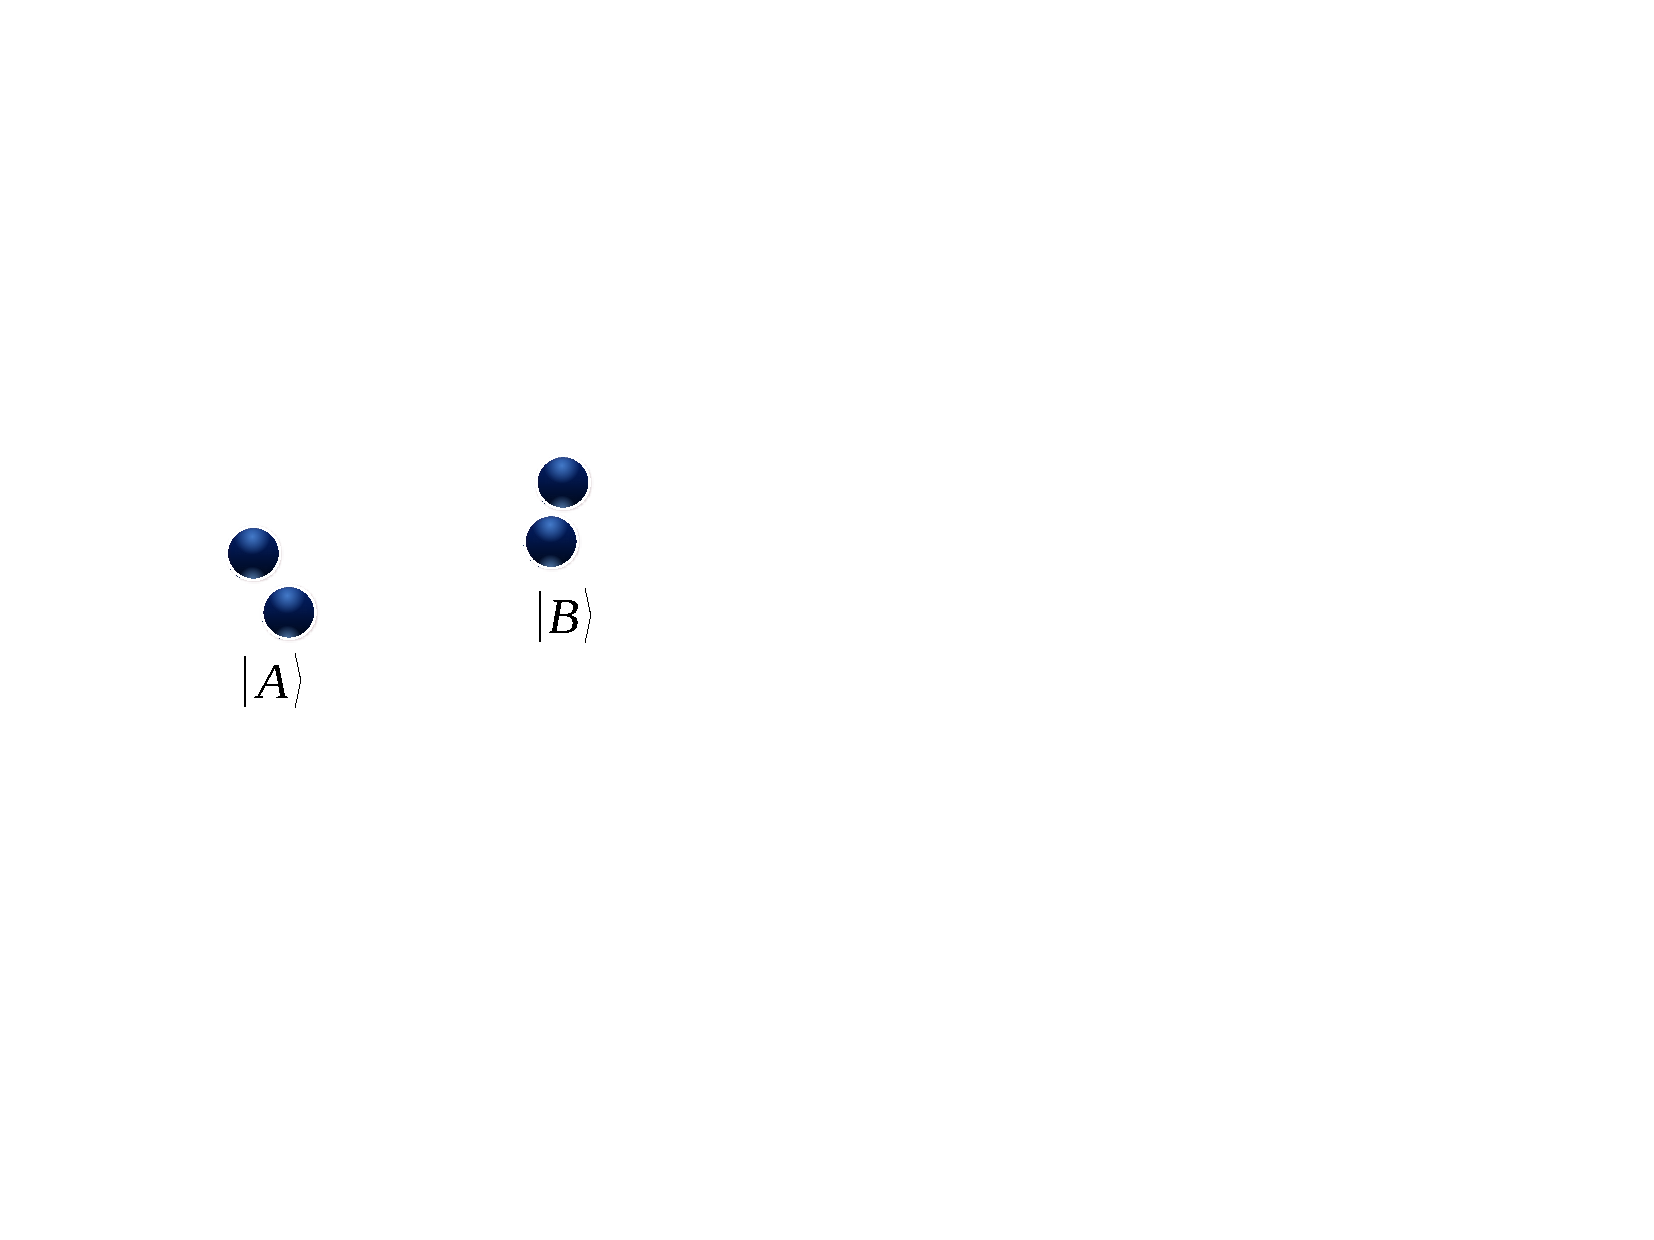
\includegraphics[width=\textwidth]{figures/cluster.pdf}
%   \caption{Energy per nucleon for ${}^4$He and ${}^{16}$O as calculated with linear, independent pair and quadratic correlations. Also, the energy per nucleon of symmetric nuclear matter of 28 particles in a periodic box with density $\rho=0.16$fm$^{-3}$. All calculations are compared to their expected values.}
%   \label{fig:cluster}
%\end{figure}

\subsection{Slater Determinant}
One of the simplest wave functions that satisfies the two properties specified above is the Slater determinant. The Slater determinant has been the starting place for a variety of many-body calculations in nuclear and condensed matter physics alike. In condensed matter the many-body wave functions will often be written in terms of a sum of weighted Slater determinants, where some methods have been able to use a sum of up to 2 billion determinants \cite{huron1973,li2018}. In nuclear physics a single determinant is often used for closed shell calculations and a sum of a small number  of weighted determinants is used for open shell systems. For small to medium mass open-shell nuclei on the order of 10 or 100 determinants are often used. A Slater determinant is an antisymmetrized product of single particle, non-interacting, wave functions
\begin{equation}
   \Psi_{SD}(\R,S) = \mathcal{A} \left[\phi_1(\r_1)\phi_2(\r_2) \ldots \phi_A(\r_A)\right] =
   \begin{vmatrix}
      \phi_1(\r_1) & \phi_1(\r_2) & \ldots & \phi_1(\r_A) \\
      \phi_2(\r_1) & \phi_2(\r_2) & \ldots & \phi_2(\r_A) \\
      \vdots & \vdots & \ddots & \vdots \\
      \phi_K(\r_1) & \phi_K(\r_2) & \ldots & \phi_K(\r_A) \\
   \end{vmatrix},
\end{equation}
where $\R$ and $S$ are the spatial and spin coordinates of the walkers, $\mathcal{A}$ is the antisymitrization operator, and the $\phi_i(\r_j)$ are the overlap of the walker positions with the model single particle states, $\braket{\r_j}{\phi_i}$. The single particle model states are made up of a radial and spin, iso-spin dependent parts,
\begin{equation}
   \phi_k = \Phi_{nj}\left[C_{c_l,m_s}^j Y_{l,m_l}(\hat{r}_i)\chi_s(s_i)\right]_{j,m_j},
\end{equation}
where $\Phi_{nj}$ is the radial part and the rest contains the spherical harmonics $Y_{l,m_l}(\hat{r}_I)$ and spin and iso-spin states where the Clebsch-Gordan coefficients ensure the correct $j$ and $m_j$ quantum numbers, and the different states are given by the index $k$. To accurately describe the wave function of an open shell nuclei each state with the correct total angular momentum, parity $J^\pi$, and isospin $T$ is included as a separate Slater determinant.
\begin{equation}
   \braket{\R S}{\Phi}_{J^\pi,T} = \sum\limits_n c_n D\{\phi_k(\r_i,s_i)\}
\end{equation}
Here the $c_n$ coefficients are variational parameters used to minimize the energy given a set of possible state configurations. One of the simplest examples of an open shell nuclei would be $^6$He whose ground state is a $J^\pi = 0^+$ state. The two protons and two of the neutrons could be in the full $(1S_{1/2})^2$ shell while the two remaining neutrons could be in the $(1P_{3/2})^2$ shell with their $m_j=\pm 3/2, \pm 1/2$ values being equal and opposite to ensure that $J=0$. This state has two possible determinants. Other possible configurations for the two remaining neutrons would be $(1P_{1/2})^2$ with one possible determinant, $(1D_{5/2})^2$ with three possible determinants, $(2S_{1/2})^2$ with one possible determinant and $(1D_{3/2})^2$ with two possible determinants giving a total of nine possible determinants. Notice that the two neutrons could be in a combination of $S$ and $D$ shells but never an $S$ and $P$ or $D$ and $P$ to ensure the parity of the state is positive. The number of determinants used for open shell nuclei will control how accurate the trial wave function is. For closed shell nuclei such as $^4$He or $^{16}$O a single Slater determinant describing the full shell configuration is sufficient.

The radial part $\Phi_{nj}$ of the single particle states are obtained as bound state solutions to the single particle Schr\"odinger equation with a Woods-Saxon potential wine-bottle potential.
\begin{equation}
   v(r) = V_s\left[\frac{1}{1+e^{(r-r_s)/a_s}} + \alpha_se^{(-r/\rho_s)^2}\right]
\end{equation}
Here the parameters, $V_s, r_s, a_s, \alpha_s$ and $\rho_s$ are variational parameters used to shape the potential to obtain a minimum in energy.

%As an illustrative example consider the deuteron. The deuteron is in a iso-spin singlet state, $\frac{1}{\sqrt{2\pi}}(\ket{pn}-\ket{np})$. To show how the model state, $\ket{\Phi}$ would be built for this I will assume all entries are 1, though in practice the could all take on different numbers to account for the different spacial and spin dependencies of the state. Let's assume that both the neutron and the proton are in a spin up state. In this case the $\Phi(k,i)$ terms, where $k,i=1,2$, would take on the following values.
%\begin{align}
%   \phi(1,1)&=(1,0,0,0)=p\uparrow_1 \\
%   \phi(2,1)&=(0,0,1,0)=n\uparrow_1 \\
%   \phi(1,2)&=(1,0,0,0)=p\uparrow_2 \\
%   \phi(2,2)&=(0,0,1,0)=n\uparrow_2
%\end{align}
%The determinant of the Slater matrix can then be written as
%\begin{equation}
%\Psi_T=\det(S)=
%\begin{vmatrix}
%    \braket{k_1}{s_1} & \braket{k_1}{s_2} \\
%    \braket{k_2}{s_1} & \braket{k_2}{s_2}
%\end{vmatrix}
%=
%\begin{vmatrix}
%    p_1 & p_2 \\
%    n_1 & n_2
%\end{vmatrix}
%=
%p_1n_2-n_1p_2,
%\end{equation}
%which is the singlet state that we wanted to start with.

The Slater determinant is a mean-field wave function and is often used with Jastrow type short range correlations.
\begin{equation}
   \braket{\R S}{\psi_T} = \bra{\R S}\prod\limits_{i<j}f(r_{ij}) \ket{\phi}_{SD}
   \label{equ:jastrow}
\end{equation}
These correlations are spin-isospin independent and depend only on the particle separation and improve upon the uncorrelated Slater determinant wave function significantly. To maintain the cluster decomposition the functions $f(r_{ij})$ must go to unity for large particle separations. In this work I have used Slater determinant wave functions with a Jastrow factor and spin-isospin dependent correlations which will be discussed in a later section.

\subsection{Pfaffian Wave Function}
Another wave function that obeys these properties is the paired Pfaffian wave function. This wave function was developed to describe Cooper pairs which form when, at low temperature, paired fermions, such as electrons or liquid $^3$He, are energetically favorable to free particles \cite{cooper1956,leggett1975}. This idea was then expanded and used to explain superconductivity as the condensation of these bosonic cooper pairs into the ground state \cite{bardeen1957,bardeen1957_2}. A Pfaffian wave function was then introduced to describe these paired systems by Bouchaud {\it et al.} in 1988 \cite{bouchaud1988}.

The BCS, or Pfaffian, pairing wave function can be written as an antisymmetrized product of pairing wave functions, thus keeping the antisymmetry of the constituent fermions explicitly. That is,
\begin{equation}
   \Psi_{BCS}(\R S) = \mathcal{A}\left[\phi(\r_1,s_1,\r_2,s_2)\phi(\r_3,s_3,\r_4,s_4)\ldots\phi(\r_{A-1},s_{A-1},\r_A,s_A)\right],
\end{equation}
where $\mathcal{A}$ is the antisymmetrization operator, $\r_i$ and $s_i$ are the walkers positions and spins, and $\phi$ are the pairing functions which can be separated into a spatial part, whose form is determined by the system, and a spin-isospin part, which are often written in terms of singlet and triplet states.

This wave function, like the Slater determinant, can be used with additional Jastrow-like correlations as in equation~\ref{equ:jastrow}.
\begin{equation}
   \braket{\R S}{\psi_T} = \bra{\R S}\prod\limits_{i<j}f(r_{ij}) \ket{\phi}_{BCS}
\end{equation}
For more information and a more detailed use and description of this wave function I refer the reader to \cite{madeira2018_diss}.

\subsection{Spin-Isospin Dependent Correlations}
The nuclear Hamiltonian has a strong dependence on spin and isospin, and to ensure good overlap with the trial wave function, the wave function must include spin-isospin dependent correlations. From here on I will be using the Slater determinant for the long-range part of the wave function. To improve on the Jastrow correlations in equation~\ref{equ:jastrow}, spin-isospin dependent correlations can be included that obey the properties of cluster decomposability and overall antisymmetry.

I have come up with two such correlations, the exponentially correlated,
\begin{equation}
   \Psi_{\text{exp}}(\R, S) = \bra{\R S}\left[\prod\limits_{i<j}f_c(r_{ij})\right] e^{\sum\limits_{i<j}\sum\limits_{p}f_p(r_{ij})\Opij}\ket{\phi}
   \label{equ:exppsi}
\end{equation}
and the symmetrized product wave functions,
\begin{equation}
   \Psi_{\text{SP}}(\R, S) = \bra{\R S}\left[\prod\limits_{i<j}f_c(r_{ij})\right] \left[\mathcal{S}\prod\limits_{i<j}\left(1+\sum\limits_p\fpij\Opij\right)\right] \ket{\phi}.
   \label{equ:prodpsi}
\end{equation}
where the $S$ is the symmetrization operator, the $f_c(r_{ij})$ are the same Jastrow correlations as before, and the $\Opij$ are the operators from the AV6' potential, $(1,\si\cdot\sj,S_{ij})\otimes(1,\ti\cdot\tj)$, where the tensor term is $S_{ij} = 3\si\cdot\hat{r}_{ij}\sj\cdot\hat{r}_{ij}-\si\cdot\sj$. The $f_p(r_{ij})$ functions contain variational parameters and the functional form is determined by solving a Schr\"odinger-type equation with the constraint that the wave function be continuous at the healing distance \cite{pandharipande1979,pandharipande1977}.

The exponentially correlated wave function obeys cluster decomposition as long as the correlating functions, $f_p(r_{ij})$ go to zero as the particle separation increases. This dampens out nonphysical long-range particle correlations between physically separated systems. Also, due to the sum over particle pairs in the exponential, no explicit symmetrization is needed.

The symmetrized product wave function, introduced by Pandharipande and Wiringa in 1979 \cite{pandharipande1979}, requires an explicit symmetrization and is not obviously cluster decomposable. The $f_p(r_{ij})$ functions approach zero as particle separation increases and so the additional 1 is needed to maintain cluster decomposability.

When expanded to linear order the exponential and symmetrized product correlations are identical and can be written as
\begin{equation}
   \ket{\psi_T}_\text{lin} = \left[\prod\limits_{i<j}f_c(r_{ij})\right] \left(1+\sum\limits_{i<j}\sum\limits_p\fpij\Opij\right) \ket{\phi}.
\end{equation}
These correlations are symmetric, allowing for the full wave function to be antisymmetric, however it has lost the cluster decomposability in the approximation. This is because they take the form of summed, not a product of pair correlations. For higher orders expansions these two wave functions differ by commutation relations as well as the inclusion of additional correlation pairs. Until recently, only correlations up to linear order in the expansion were used for AFDMC calculations. Calculations for GFMC use a much better wave function, but have been limited to small nuclei up to $^{12}$C. Calculations done with the AFDMC method have been slowly improving the trial wave function used, as a better wave function is surely needed to describe larger systems. In 2007 AFDMC binding energy calculations were done for $^4$He, $^{16}$O, and $^{40}$Ca using only the Jastrow correlations \cite{gandolfi2007}. These calculations were repeated in 2014 but with the addition of linear correlations \cite{gandolfi2014} and I have plotted the respective results compared to current experimental values here for comparison.
\begin{figure}[h!]
   \centering
   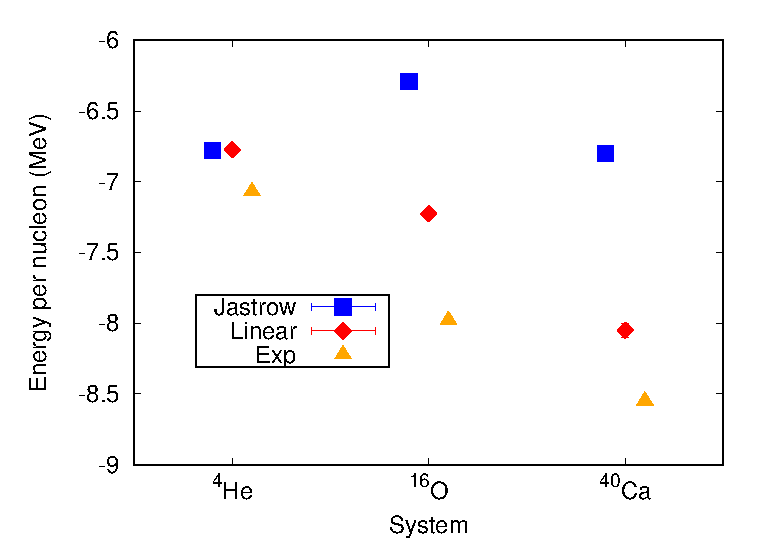
\includegraphics[width=0.7\textwidth]{figures/energy_jaslin.eps}
   \caption{Binding energy calculations done with Jastrow correlations \cite{gandolfi2007} compared to Jastrow plus linear spin-isospin dependent correlations \cite{gandolfi2014} all compared to experimental results. All calculations were done with AFDMC and the AV6$'$ potential.}
   \label{fig:energy_jaslin}
\end{figure}
In figure~\ref{fig:energy_jaslin} it is clear to see that the additional spin-isospin correlations are important for both systems larger than $^4$He.

\subsubsection{Quadratic Correlations}
In this project I have included correlations up to quadratic order which includes up to 4 nucleons begin correlated at once. When expanded to quadratic order the symmetrized product wave function, equation~\ref{equ:prodpsi}, becomes
\begin{equation}
   \begin{split}
      \ket{\psi_T}_\text{quad} = \Bigg[\prod\limits_{i<j}&f_c(r_{ij})\Bigg] \Bigg[1+\fOpij \\
         & + \frac{1}{2}\fOpij\fOqklquad \Bigg] \ket{\phi}.
   \end{split}
   \label{equ:fullquadcorr}
\end{equation}
The subscripts on the sums, which describe which correlations are allowed, can be hard to visualize and so these correlation diagrams are useful.
\begin{figure}[h]
\newcommand\shift{2.0}
\newcommand\vshift{-1.5} %vertical shift
\newcommand\tshift{0.05} %tiny shift
\newcommand\sep{0.75}
   \centering
   \begin{tikzpicture}[>=latex,scale=1.0]
      \draw (-2*\sep,\sep/2.0) node{\large Allowed};
      \draw (-2*\sep,\sep/2.0+\vshift) node{\large Not Allowed};

      \filldraw[black] (0*\shift,0)          circle (2pt) node[anchor=east] {\large j};
      \filldraw[black] (0*\shift,\sep)       circle (2pt) node[anchor=east] {\large i};
      \filldraw[black] (0*\shift+\sep,0)     circle (2pt) node[anchor=west] {\large l};
      \filldraw[black] (0*\shift+\sep,\sep)  circle (2pt) node[anchor=west] {\large k};
      \draw[black, ultra thick] (0*\shift,\sep) -- (0*\shift,0); %i-j
      \draw[black, ultra thick] (0*\shift+\sep,\sep) -- (0*\shift+\sep, 0); %k-l

      \filldraw[black] (1*\shift,0)          circle (2pt) node[anchor=east] {\large k};
      \filldraw[black] (1*\shift,\sep)       circle (2pt) node[anchor=east] {\large i};
      \filldraw[black] (1*\shift+\sep,0)     circle (2pt) node[anchor=west] {\large l};
      \filldraw[black] (1*\shift+\sep,\sep)  circle (2pt) node[anchor=west] {\large j};
      \draw[black, ultra thick] (1*\shift,\sep) -- (1*\shift+\sep,\sep); %i-j
      \draw[black, ultra thick] (1*\shift,0) -- (1*\shift+\sep,0); %k-l

      \filldraw[black] (2*\shift,0)          circle (2pt) node[anchor=east] {\large l};
      \filldraw[black] (2*\shift,\sep)       circle (2pt) node[anchor=east] {\large i};
      \filldraw[black] (2*\shift+\sep,0)     circle (2pt) node[anchor=west] {\large j};
      \filldraw[black] (2*\shift+\sep,\sep)  circle (2pt) node[anchor=west] {\large k};
      \draw[black, ultra thick] (2*\shift,\sep) -- (2*\shift+\sep,0); %i-j
      \draw[black, ultra thick] (2*\shift+\sep,\sep) -- (2*\shift,0); %k-l

      \filldraw[black] (3*\shift,0)          circle (2pt) node[anchor=east] {\large j};
      \filldraw[black] (3*\shift,\sep)       circle (2pt) node[anchor=east] {\large i,k};
      \filldraw[black] (3*\shift+\sep,0)     circle (2pt) node[anchor=west] {\large };
      \filldraw[black] (3*\shift+\sep,\sep)  circle (2pt) node[anchor=west] {\large l};
      \draw[black, ultra thick] (3*\shift,\sep) -- (3*\shift,0); %i-j
      \draw[black, ultra thick] (3*\shift,\sep) -- (3*\shift+\sep,\sep); %k-l

      \filldraw[black] (4*\shift,0)          circle (2pt) node[anchor=east] {\large k};
      \filldraw[black] (4*\shift,\sep)       circle (2pt) node[anchor=east] {\large i};
      \filldraw[black] (4*\shift+\sep,0)     circle (2pt) node[anchor=west] {\large j,l};
      \filldraw[black] (4*\shift+\sep,\sep)  circle (2pt) node[anchor=west] {\large };
      \draw[black, ultra thick] (4*\shift,\sep) -- (4*\shift+\sep,0); %i-j
      \draw[black, ultra thick] (4*\shift,0) -- (4*\shift+\sep,0); %k-l

      \filldraw[black] (2*\shift,\vshift)             circle (2pt) node[anchor=east] {\large j,l};
      \filldraw[black] (2*\shift,\sep+\vshift)        circle (2pt) node[anchor=east] {\large i,k};
      \filldraw[black] (2*\shift+\sep,\vshift)        circle (2pt) node[anchor=west] {\large };
      \filldraw[black] (2*\shift+\sep,\sep+\vshift)   circle (2pt) node[anchor=west] {\large };
      \draw[black, ultra thick] (2*\shift-\tshift,\sep+\vshift) -- (2*\shift-\tshift,\vshift); %i-j
      \draw[black, ultra thick] (2*\shift+\tshift,\sep+\vshift) -- (2*\shift+\tshift,\vshift); %k-l
   \end{tikzpicture}
   \caption{Diagrams used to visualize which correlations are included in the quadratic correlations in equation~\ref{equ:fullquadcorr}.}
   \label{fig:quaddiagrams}
\end{figure}
All pair correlations are included in this wave function except pairs that are directly correlated with themselves, e.g. $\mathcal{O}_{23}\mathcal{O}_{23}$, where $\mathcal{O}_{ij}$ is a product of single particle operators such as $\si\cdot\sj$ and $\mathcal{O}_{ij}=\mathcal{O}_{ji}$ due to the operators on different particles operating in different Hilbert spaces. For correlations where the same particle is included twice, the correlation operators do not commute and that term must be explicitly symmetrized. Currently in equation~\ref{equ:fullquadcorr} and in the code all quadratic terms are symmetrized, e.g. the correlation $\mathcal{O}_{12}\mathcal{O}_{34}$ is symmetrized as $\frac{1}{2}\left(\mathcal{O}_{12}\mathcal{O}_{34}+\mathcal{O}_{34}\mathcal{O}_{12}\right)$, even though only terms like $\mathcal{O}_{12}\mathcal{O}_{13}$ need this explicit symmetrization. This adds needless calculation time, but as I'll show, these terms don't seem to be significant and can be omitted completely.

If the exponentially correlated wave function, equation~\ref{equ:exppsi}, is expanded in the typical way, i.e. $\exp(A) = 1 + A + \frac{1}{2}A^2 + \ldots$, then the quadratic correlations for the exponential wave function become
\begin{equation}
   \begin{split}
      \ket{\psi_T}_\text{exp\_quad} = \Bigg[\prod\limits_{i<j}&f_c(r_{ij})\Bigg] \Bigg[1+\fOpij \\
         & + \frac{1}{2}\fOpij\fOqklexpquad \Bigg] \ket{\phi}.
   \end{split}
   \label{equ:expquadcorr}
\end{equation}
Unlike the quadratic correlations derived from the symmetrized product this wave function includes all of the the terms in figure~\ref{fig:quaddiagrams}. There is not a large difference between these wave functions up to quadratic order and for here forward all references to quadratic correlations will refer to the expansion from the symmetrized product wave function.

Another way to include quadratic correlations is to only include terms that do not correlate the same particle twice leaving only independent pair correlations. This is the same whether you start from the exponentially correlated or the symmetrized product wave function and it can be written as
\begin{equation}
   \begin{split}
      \ket{\psi_T}_\text{ip} = \Bigg[\prod\limits_{i<j}&f_c(r_{ij})\Bigg] \Bigg[1+\fOpij \\
      & + \fOpij\fOqklip \Bigg] \ket{\phi}
   \end{split}
   \label{equ:ipquadcorr}
\end{equation}
and the independent pair sum can be visualized as in figure~\ref{fig:ipdiagrams}.
\begin{figure}[h]
\newcommand\shift{2.2}
\newcommand\vshift{-1.5} %vertical shift
\newcommand\tshift{0.05} %tiny shift
\newcommand\sep{0.75}
   \centering
   \begin{tikzpicture}[>=latex,scale=1.0]
      \draw (-3*\sep,\sep/2.0) node{\large Allowed};
      \draw (-3*\sep,\sep/2.0+\vshift) node{\large Not Allowed};

      \filldraw[black] (0*\shift,0)          circle (2pt) node[anchor=east] {\large j};
      \filldraw[black] (0*\shift,\sep)       circle (2pt) node[anchor=east] {\large i};
      \filldraw[black] (0*\shift+\sep,0)     circle (2pt) node[anchor=west] {\large l};
      \filldraw[black] (0*\shift+\sep,\sep)  circle (2pt) node[anchor=west] {\large k};
      \draw[black, ultra thick] (0*\shift,\sep) -- (0*\shift,0); %i-j
      \draw[black, ultra thick] (0*\shift+\sep,\sep) -- (0*\shift+\sep, 0); %k-l

      \filldraw[black] (1*\shift,0)          circle (2pt) node[anchor=east] {\large k};
      \filldraw[black] (1*\shift,\sep)       circle (2pt) node[anchor=east] {\large i};
      \filldraw[black] (1*\shift+\sep,0)     circle (2pt) node[anchor=west] {\large l};
      \filldraw[black] (1*\shift+\sep,\sep)  circle (2pt) node[anchor=west] {\large j};
      \draw[black, ultra thick] (1*\shift,\sep) -- (1*\shift+\sep,\sep); %i-j
      \draw[black, ultra thick] (1*\shift,0) -- (1*\shift+\sep,0); %k-l

      \filldraw[black] (2*\shift,0)          circle (2pt) node[anchor=east] {\large l};
      \filldraw[black] (2*\shift,\sep)       circle (2pt) node[anchor=east] {\large i};
      \filldraw[black] (2*\shift+\sep,0)     circle (2pt) node[anchor=west] {\large j};
      \filldraw[black] (2*\shift+\sep,\sep)  circle (2pt) node[anchor=west] {\large k};
      \draw[black, ultra thick] (2*\shift,\sep) -- (2*\shift+\sep,0); %i-j
      \draw[black, ultra thick] (2*\shift+\sep,\sep) -- (2*\shift,0); %k-l

      \filldraw[black] (0*\shift,\vshift)          circle (2pt) node[anchor=east] {\large j};
      \filldraw[black] (0*\shift,\sep+\vshift)       circle (2pt) node[anchor=east] {\large i,k};
      \filldraw[black] (0*\shift+\sep,\vshift)     circle (2pt) node[anchor=west] {\large };
      \filldraw[black] (0*\shift+\sep,\sep+\vshift)  circle (2pt) node[anchor=west] {\large l};
      \draw[black, ultra thick] (0*\shift,\sep+\vshift) -- (0*\shift,\vshift); %i-j
      \draw[black, ultra thick] (0*\shift,\sep+\vshift) -- (0*\shift+\sep,\sep+\vshift); %k-l

      \filldraw[black] (1*\shift,\vshift)          circle (2pt) node[anchor=east] {\large k};
      \filldraw[black] (1*\shift,\sep+\vshift)       circle (2pt) node[anchor=east] {\large i};
      \filldraw[black] (1*\shift+\sep,\vshift)     circle (2pt) node[anchor=west] {\large j,l};
      \filldraw[black] (1*\shift+\sep,+\vshift)  circle (2pt) node[anchor=west] {\large };
      \draw[black, ultra thick] (1*\shift,\sep+\vshift) -- (1*\shift+\sep,\vshift); %i-j
      \draw[black, ultra thick] (1*\shift,\vshift) -- (1*\shift+\sep,\vshift); %k-l

      \filldraw[black] (2*\shift,\vshift)             circle (2pt) node[anchor=east] {\large j,l};
      \filldraw[black] (2*\shift,\sep+\vshift)        circle (2pt) node[anchor=east] {\large i,k};
      \filldraw[black] (2*\shift+\sep,\vshift)        circle (2pt) node[anchor=west] {\large };
      \filldraw[black] (2*\shift+\sep,\sep+\vshift)   circle (2pt) node[anchor=west] {\large };
      \draw[black, ultra thick] (2*\shift-\tshift,\sep+\vshift) -- (2*\shift-\tshift,\vshift); %i-j
      \draw[black, ultra thick] (2*\shift+\tshift,\sep+\vshift) -- (2*\shift+\tshift,\vshift); %k-l
   \end{tikzpicture}
   \caption{Diagrams used to visualize which correlations are included in the independent pair quadratic correlations in equation~\ref{equ:ipquadcorr}.}
   \label{fig:ipdiagrams}
\end{figure}
All terms where a particle is included twice in the correlation are ignored, as a results, all correlation operators commute and the correlations are explicitly symmetric. Neither of these correlations maintains cluster decomposability, however an effort to build an antisymmetric and cluster decomposable wave function from the exponentially correlated wave function will be discussed later.

The energy and it's uncertainty are used to judge the convergence of a propagated wave function in QMC and so a good wave function needs to be able to reproduce known binding energies. To this end I have calculated binding energies with the linear, quadratic, and independent pair (IP) quadratic correlations derived from the symmetrized product for $^4$He, $^{16}$O, $^{40}$Ca, and symmetric nuclear matter (SNM) at saturation density, $\rho_0=0.16$ fm$^{-3}$, in a period box with 28 particles. The energy per particle for nuclei is plotted in figure~\ref{fig:energies} and the specific energies can be found in table~\ref{tab:energies}.
\begin{figure}[h!]
   \centering
   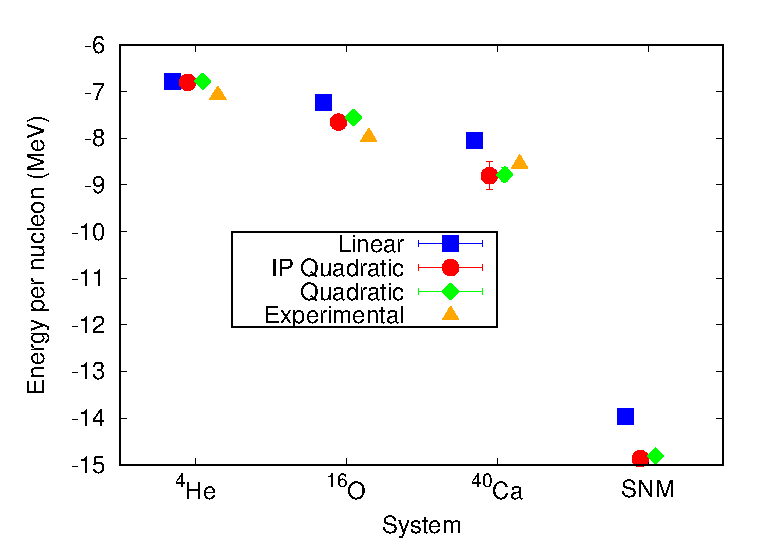
\includegraphics[width=0.7\textwidth]{figures/energy.eps}
   \caption{Energy per particle for small and medium closed shell nuclei with no Coulomb interaction with the AV6$'$ interaction. Each calculations was done with the linear, independent pair, and quadratic correlations. Energies are compared to experimental values where available and the statistical uncertainties are included.}
   \label{fig:energies}
\end{figure}
\begin{table}[htb]
   \centering
   \begin{tabular}{ccccc}
      \hline\hline
      System & Linear & Ind-Pair & Quadratic & Experimental \\
      \hline
      $^4${He}    & -6.785(10)   & -6.798(8) & -6.778(8)    & -7.074 \\   
      $^{16}${O}  & -7.23(6)     & -7.65(9)  & -7.55(8)     & -7.98  \\   
      $^{40}${Ca} & -8.05(8)     & -8.8(3)   & -8.78(15)    & -8.55  \\
      SNM         & -13.97(3)    & -14.87(4) & -14.70(11)   &        \\
      \hline\hline
   \end{tabular}
   \label{tab:energies}
   \caption{Energy per particle calculated with no Coulomb interaction with the AV6$'$ interaction. Each calculations was done with the linear, independent pair, and quadratic correlations. Energies are compared to experimental values where available and the statistical uncertainties are included.}
\end{table}
Like with the addition of Jastrow correlations in figure~\ref{fig:energy_jaslin}, all systems larger than $^4$He decreased in energy with additional correlations, while the binding energy for $^4$He was the same to within uncertainties. In addition, the energies for all systems are identical to within uncertainties for the quadratic and IP quadratic correlations, indicating that the IP correlations capture most of the relevant physics. As a result any further references to quadratic correlations will be referring to the IP quadratic correlations, as these correlations are computationally less expensive, unless a distinction is made otherwise. The percent decrease in energy for $^{16}$O and $^{40}$Ca when adding linear correlations is 15\% and 18\% respectively. When adding quadratic correlations the energies decrease an additional 6\% and 9\% respectively. This indicates that each successive term in the expansion decreases in importance.

There is a significant decrease in energy with the addition of the quadratic correlations, however, there is an additional cost to calculating these additional terms. I have calculated a scaling factor, which is the ratio of times taken to calculate a given block of code, including the propagation of walkers spatial and spin components as well as the calculation of the energies, for linear compared to linear plus quadratic correlations. A scaling factor of 2 would mean that the calculation took twice as long with the quadratic correlations as it did without. The scaling factors are plotted in figure~\ref{fig:scaling} and the specific values are in table~\ref{tab:scaling}.
\begin{figure}[h!]
   \centering
   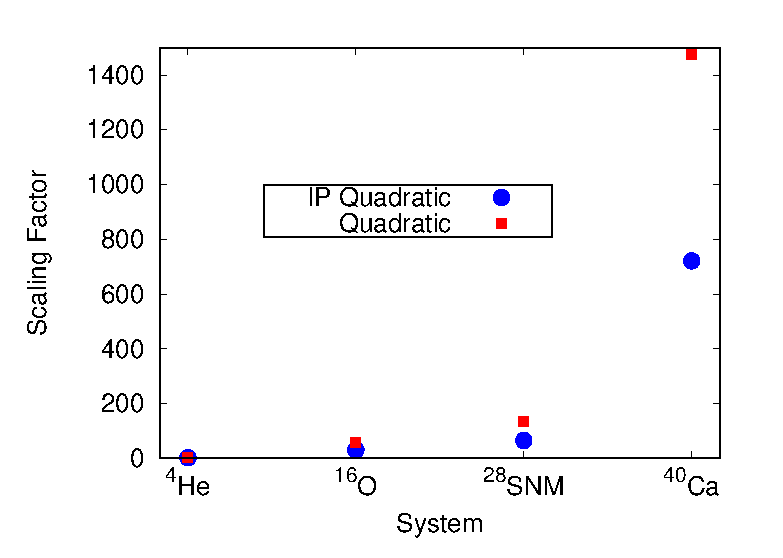
\includegraphics[width=0.7\textwidth]{figures/scaling.eps}
   \caption{Scaling factors calculated as the ratio of times taken to calculate a given block of code for linear and linear plus quadratic correlations.}
   \label{fig:scaling}
\end{figure}
\begin{table}[htb]
   \centering
   \begin{tabular}{ccccc}
      \hline \hline
       & $^{4}$He & $^{16}$O & SNM(28) & $^{40}$Ca \\
      \hline
      IP Quadratic & 1.73 & 30.7 & 64.8 & 720.9 \\
      Quadratic & 2.00 & 58.8 & 133.6 & 1473.9 \\
      \hline \hline
   \end{tabular}
   \label{tab:scaling}
   \caption{Same scaling factors that are calculated in figure~\ref{fig:scaling}.}
\end{table}
The scaling for the quadratic correlations is about twice that of the IP quadratic correlations. This is due to the explicit symmetrization that is done for each quadratic term in the quadratic correlations. This could be decreased if commuting terms were not symmetrized, however as noted before the IP quadratic correlations seem to capture the important physics, and so all future calculations with quadratic correlations will be using the IP correlations. The IP correlations all commute and so no explicit symmetrization is needed. A typical AFDMC calculation using only linear correlations for $^{16}$O with 1000 walkers takes on the order of a tens of CPU hours and a similar calculation for $^{40}$Ca takes on the order of hundreds of CPU hours.

The number of quadratic terms in the IP correlations given $A$ particles is
\begin{equation}
   N_\text{ip}=\frac{A(A-1)(A-2)(A-3)}{8}.
\end{equation}
For the fully quadratic wave function the number of terms given $A$ particles is
\begin{equation}
   N_\text{quad}=\frac{A(A-1)}{2}\left(\frac{A(A-1)}{2}-1)\right),
\end{equation}
where $A(A-1)/2$ is the number of possible pairs made from $A$ particles. If the fully quadratic correlations are not explicitly symmetrized for the IP terms then this reduces to $N_\text{quad}-N_\text{ip}$. In figure~\ref{fig:scaling_theory} I have plotted the number of terms for the independent pair, fully quadratic, and fully quadratic correlations without symmetrizing the IP terms.
\begin{figure}[h!]
   \centering
   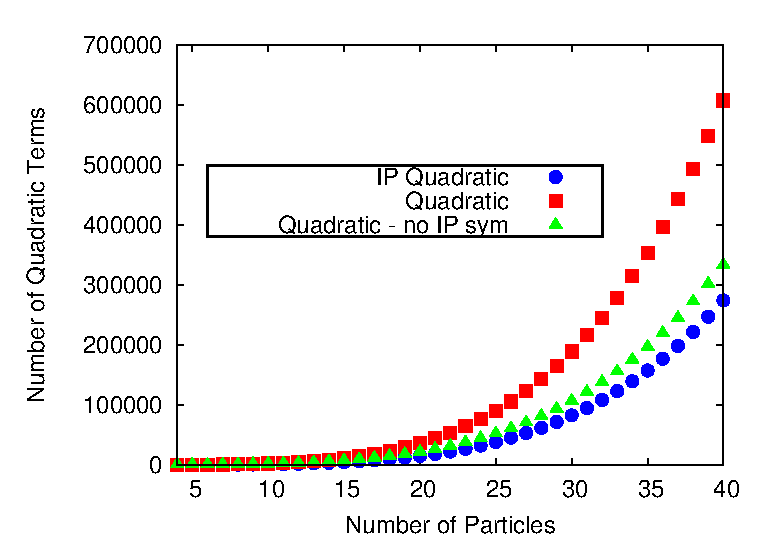
\includegraphics[width=0.7\textwidth]{figures/scaling_theory.eps}
   \caption{Number of terms in the quadratic correlations for the IP, quadratic, and quadratic correlations without explicit symmetrization of the IP terms.}
   \label{fig:scaling_theory}
\end{figure}

In recent years efforts have been made to fit infinite matter saturation properties with microscopic nuclear interactions \cite{drischler2017}. Calculations of energies near saturation using AFDMC have not been able to fit known saturation properties. I have done calculations of symmetric nuclear matter near saturation with and without quadratic correlations, using only the AV6$'$ 2-body interaction and have compared these results to known saturation properties in figure~\ref{fig:saturation}. Though 3N forces will surely be needed to obtain a good fit, it is clear that improved correlations are also going to be needed.
\begin{figure}[h!]
   \centering
   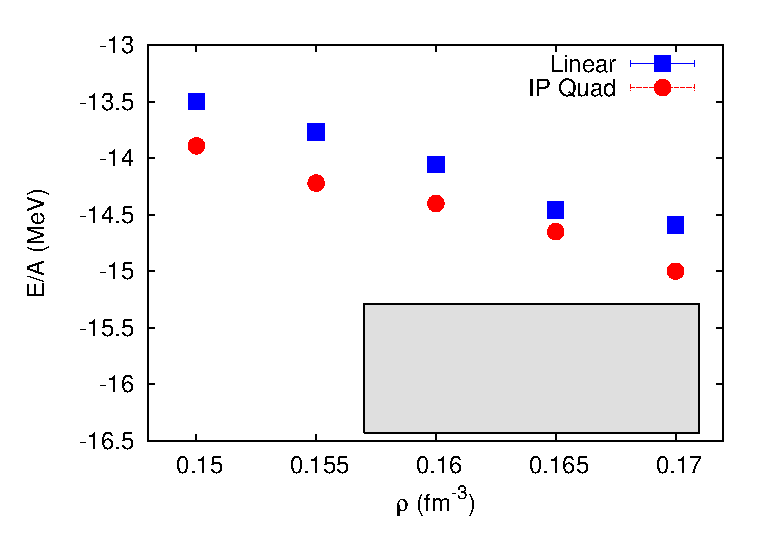
\includegraphics[width=0.7\textwidth]{figures/saturation.eps}
   \caption{Energy calculations done using the AV6$'$ potential with linear and quadratic correlations. The gray box is the same empirical saturation region used in \cite{drischler2017}, $\rho_0 = 0.164 \pm 0.007$ fm$^{-3}$ and $E/A=-15.86 \pm 0.57$ MeV.}
   \label{fig:saturation}
\end{figure}

\subsubsection{Exponential Correlations}
From the wave function using the expansion up to quadratic terms it is clear that an improved trial wave function is necessary to describe the state of larger nuclei and nuclear matter. It was also shown in the previous sections that expanding the current wave functions, Equations~\ref{equ:exppsi} and \ref{equ:prodpsi} is not an efficient method to improve the wave function, as the cost of each additional term grows exponentially. However, another option is to evaluate the full wave function using a Monte Carlo sampling. The exponential wave function is written as
\begin{equation}
   \ket{\Psi_T} = \left[\prod\limits_{i<j}f_c(r_{ij})\right] e^{\sum\limits_{i<j,p}f_p(r_{ij})\Oijp} \ket{\Phi},
\end{equation}
which has the same operator form as the spin-isospin propagator used in AFDMC, where again, the operators are the AV6$'$ operators, $\si\cdot\sj$, $\ti\cdot\tj$, $\si\cdot\sj \ti\cdot\tj$, $S_{ij}$ and $S_{ij} \ti\cdot\tj$, where $S_{ij} = 3\si\cdot\hat{r}_{ij}\sj\cdot\hat{r}_{ij}-\si\cdot\sj$. These operators are written in terms of squared single particle operators, allowing for the Hubbard Stratanovich transformation to express the correlations in terms of a single particle operator and integrals over auxiliary fields, which are evaluated via Monte Carlo.

The correlation functions $f_p(r_{ij})$ are written in terms of symmetric matrices
\begin{equation}
   \exp\left(\sum\limits_{i<j,p}f_p(r_{ij})\Oijp\right) = \exp\left(\frac{1}{2}\sum\limits_{i\alpha,j\beta} \sigma_{i\alpha}A^{\sigma}_{i\alpha,j\beta}\sigma_{j\beta}
      + \frac{1}{2}\sum\limits_{i\alpha,j\beta} \sigma_{i\alpha}A^{\sigma\tau}_{i\alpha,j\beta}\sigma_{j\beta}\ti\cdot\tj
      + \frac{1}{2}\sum\limits_{i,j} A^{\tau}_{i,j}\ti\cdot\tj\right),
\end{equation}
which can be written in terms of their eigenvalues and eigenvectors
\begin{align}
   &\sum\limits_{j\beta} A^{\sigma}_{i\alpha,j\beta}\psi^{\sigma}_{n,j\beta} = \lambda^{\sigma}_n\psi^{\sigma}_{n,i\alpha} \\
   &\sum\limits_{j\beta} A^{\sigma\tau}_{i\alpha,j\beta}\psi^{\sigma\tau}_{n,j\beta} = \lambda^{\sigma\tau}_n\psi^{\sigma\tau}_{n,i\alpha} \\
   &\sum\limits_{j} A^{\tau}_{i,j}\psi^{\tau}_{n,j} = \lambda^{\tau}_n\psi^{\tau}_{n,i}.
\end{align}
The correlations are then written in terms of squared single particle operators,
\begin{equation}
   \exp\left(\sum\limits_{i<j,p}f_p(r_{ij})\Oijp\right) = \exp\left(\frac{1}{2}\sum\limits_{n=1}^{3A} \left(O_{n}^{\sigma}\right)^2 \lambda_n^{\sigma}
      + \frac{1}{2}\sum\limits_{\alpha=1}^{3}\sum\limits_{n=1}^{3A} \left(O_{n\alpha}^{\sigma\tau}\right)^2 \lambda_n^{\sigma\tau}
      + \frac{1}{2}\sum\limits_{\alpha=1}^{3}\sum\limits_{n=1}^{A} \left(O_{n\alpha}^{\tau}\right)^2 \lambda_n^{\tau}\right),
\end{equation}
where the operators are given by
\begin{equation}
\begin{split}
   O_{n}^{\sigma} &= \sum\limits_{j,\beta} \sigma_{j,\beta}\psi_{n,j,\beta}^{\sigma} \\
   O_{n\alpha}^{\sigma\tau} &= \sum\limits_{j,\beta} \tau_{j,\alpha}\sigma_{j,\beta}\psi_{n,j,\beta}^{\sigma\tau} \\
   O_{n\alpha}^{\tau} &= \sum\limits_{j} \tau_{j,\alpha}\psi_{n,j}^{\tau}.
\end{split}
\end{equation}
This can be written in a more compact form,
\begin{equation}
    \exp\left(\sum\limits_{i<j,p}f_p(r_{ij})\Oijp\right) = \exp\left(\frac{1}{2}\sum\limits_{n=1}^{15A} \left(O_{n}\right)^2 \lambda_n^{\sigma}\right).
\end{equation}
The Hubbard Stratanovich transformation is then used to write these as single particle operators and integrals over auxiliary fields, $x_n$. Ignoring commutator terms this can be written as
\begin{equation}
   \exp\left(\frac{1}{2}\sum\limits_{n=1}^{15A} \left(O_{n}\right)^2 \lambda_n^{\sigma}\right) = \prod\limits_{n=1}^{15A} \frac{1}{\sqrt{2\pi}}\int dx_n e^{-x_n^2/2}e^{\sqrt{\lambda_n}x_nO_n}.
\end{equation}

The auxiliary fields are then drawn from the Gaussian distribution, $\exp\left(-x_n^2/2\right)$ and the correlations can be written as
\begin{equation}
   \Psi_T(R,S) = \bra{RS}\prod\limits_{n=1}^{15A} \frac{1}{N} \sum\limits_{\{x_n\}}^N\frac{1}{\sqrt{2\pi}}e^{\sqrt{\lambda_n}x_nO_n}\ket{\Phi}.
\end{equation}
The $\{x_n\}$ are the set of 15$A$ auxiliary fields, one for each of the different 15$A$ operators.

Minimal success has been achieved with these correlations for light nuclei \cite{bouadani2009_dissertation}, however there are large uncertainties that make this wave function currently infeasible to use. Removing these uncertainties could make this wave function a very useful tool for nuclear QMC as it can be systematically improved by increasing the number of samples of the auxiliary fields.

One difference between this wave function and the propagator used in AFDMC is the lack of a small time step. This wave function contains no time step and so there is no way to ensure that commutator terms will be small. Another possible issue arises when evaluating the derivative in the kinetic energy. The shifting of the walker positions causes the $A$ matrices to be discontinuous, and thus causing large uncertainties in the calculation of the derivative.

\subsubsection{Alessandro's correlations and $T^2$ fix to them - \red{Maybe just do $T^2$ fix and apply it to exponential correlations \ldots maybe don't include this at all.}}
